\documentclass[12pt]{article}
%% \usepackage{bookman}
\usepackage{hyperref}
\usepackage{amsfonts}
\usepackage{amsmath}
\usepackage{graphicx}
\usepackage{sidecap}
\usepackage[numbers]{natbib} 
\usepackage[font=small,labelfont=sf, margin=1in]{caption}
\usepackage{rotating}

\hypersetup{
  % bookmarks=true,         % show bookmarks bar?
    unicode=false,          % non-Latin characters in Acrobat’s bookmarks
    pdftoolbar=true,        % show Acrobat’s toolbar?
    pdfmenubar=true,        % show Acrobat’s menu?
    pdffitwindow=false,     % window fit to page when opened
    pdfstartview={FitH},    % fits the width of the page to the window
    pdftitle={Thesis Proposal},
    pdfauthor={Wei Liu},     % author
    pdfsubject={Wei Liu's Thesis Proposal},   % subject of the document
    pdfcreator={Wei Liu},   % creator of the document
    pdfproducer={Wei Liu}, % producer of the document
    pdfkeywords={Thesis Proposal, fmri, functional brain connectivity}, % list of keywords
    pdfnewwindow=true,      % links in new window
    colorlinks= true,       % false: boxed links; true: colored links
    linkcolor=blue,          % color of internal links
    citecolor=blue,        % color of links to bibliography
    filecolor=magenta,      % color of file links
    urlcolor=cyan           % color of external links
}

\setlength{\oddsidemargin}{0 in}
\setlength{\evensidemargin}{0 in}
\setlength{\topmargin}{-1 in}
\setlength{\textwidth}{6.5 in}
\setlength{\textheight}{9 in}
\setlength{\headsep}{0.5 in}
\setlength{\parindent}{0 in}
\setlength{\parskip}{0.1 in}

\begin{document}
\title{Thesis Proposal}
\author{Wei Liu}
%% \author{Wei Liu\\ \small{(advisor: Tom Fletcher)} }
\date{\today} 

\maketitle 

\section{Introduction}

Resting-state functional MRI (rs-fMRI) is increasingly used for probing
functional connectivity of the human brain. The spontaneous activity identified
by rs-fMRI plays a key role in understanding the normal brain's functional
organization. It also holds valuable diagnostic and prognostic information
towards various neurological or psychiatric diseases including Alzheimer's
disease, depression, schizophrenia, etc~\cite{fox2007spontaneous}. The blood
oxygenation level-dependent (BOLD) signal of fMRI detects the locations of
increased neuro activity by measuring the blood oxygen levels at consecutive
time points. The higher the temporal correlation between two spatially distant
regions, the more likely that there is a functional connection between those
regions.

The analysis of rs-fMRI data is a challenging task, due to the scanner noise,
physiological noise, head motion, and subject's random thoughts during data
acquisition. Various techniques are proposed to address these issue. Among them,
(1) spatial smoothing is used to increase the signal-to-noise ratio, and (2)
group analysis is used to increase the statistical power by estimating an
average functional network and to allow comparisons between groups. Both
approaches have drawbacks that are to be elaborated in the next two paragraphs.
In my work I address the issues concerning the above two aspects, with the focus
on the latter.

In conventional functional connectivity studies, the spatial regularities of the
connectivity are enforced by applying a smoothing filter as a preprocessing
step. Depending on the noise level and the number of subjects in a group study,
optimal kernel width of the filter may vary~\cite{mikl2008effects}. In current
state-of-art processing pipeline, the kernel size is arbitrarily given a value
ranging from 4mm to 10mm. This may introduce over-smoothing and pose difficulty
in identifying connections between small regions, or introduce under-smoothing
resulting in insufficient noise reduction. Moreover, the sub-optimal choice of
the smoothing parameters can change the result drastically. There needs to be a
statistical method that explicitly models the spatial smoothness of the
connectivity patterns. The model should be data-driven in that the parameters
are estimated from the fMRI images data under study.

In the group analysis, subjects may exhibit similar but not exactly same
spontaneous BOLD fluctuation. Current group studies typically first identify
each subject's connectivity separately regardless of other subjects, and then
estimate a \emph{pooled} summary of the group connectivity
map~\cite{van2008normalized,craddock2011whole}, or estimate group map first and
then back-reconstruct the subject network map~\cite{calhoun2001method}.  Such
approaches are sub-optimal, since estimation of one subject's connectivity does
not benefit from other subjects. From a Bayesian  point of view, once
the population distribution is known, it can help each subject's estimation as a
prior. Subjects network estimates also gives feedback on group estimation.  We
need a data-driven, unified probabilistic framework and put the connectivity
variables of both group and subjects jointly into this model. Inference can be
made from the posterior of the variables in both (subject and group) levels
given the observed time series data.

Furthermore, the full Bayesian model provides us an opportunity to study the
variability of the functional network by inference of the posterior. Besides the
traditional variance and confidence interval analysis, the mode of spatial
variability can be inferred from multivariate analysis. For the first time, to
our best knowledge, it would be possible to visualize how functional homogeneous
regions change along the principal direction of their posterior variability, and
compare these change across subjects.

\section{Thesis Statement}

\begin{center}
\parbox{5in}{\emph{\textbf{A multilevel Markov Random Field model improves the
      reliability of the functional network estimation in rs-fMRI group study by
      taking into account context information as a prior. The data-driven
      Bayesian model can jointly estimate both population and subjects'
      connectivity networks, as well as drawing inference on the uncertainty in
      the estimation, and on the variability across subjects. }}}
\end{center}

\noindent The phrase \emph{Context} has two meanings: 1) The functional patterns
of human brain is spatially coherent. Neighboring voxels have larger probability
of being in the same functional network. 2) The network that a voxel belongs to
in one subjects is dependant on the networks of the same voxels in other
subjects. The patterns of functional networks from the rs-fMRI study are to some
extent shared by multiple subjects, while the variability across subjects must
be taken into account.

By \emph{reliability} I mean the decrease in the variance of the functional
networks that we estimate with different subsets of all subjects. The reliable
estimates will be closer to the true network in simulation test, where we know
the true answer.

%% By \emph{variability} I mean the uncertainty on the size and shape of the spatial
%% patterns of the networks due to the posterior density, and due to the difference
%% between subjects.


\section{Contributions}\label{sec:cont}
To test our statement, we propose the following contributions:
\begin{itemize}
  \item \textbf{Full Pairwise Connectivity With Spatial Coherence.} I propose a
    method that estimates pairwise functional connectivity in the whole brain of
    a single subject, without \emph{a priori} knowledge of the seed region. The
    model needs to take into account the spatial context information, and learn
    the strength of the coherence from the data.

  \item \textbf{Identify Consistent, Spatially Coherent Multiple Functional
    Networks.} I propose a data-driven, generative model that can cluster the
    gray matter voxels of single subject's brain into disjoint multiple
    functional networks, while respecting the spatial coherence of the voxels.

  \item \textbf{Hierarchical Model For Group Study.} I propose a hierarchical
    model that can estimate functional networks from a group of subjects. The
    model will estimate an overall group's network map as well as individual
    subjects network maps at the same time. When Clustering the voxels into
    different networks, spatial neighbors both within and across subjects will
    be used in a prior of a Bayesian framework. The variability of each
    subject's connectivity due to noise and artifact will be reduced to the
    extent that is to be determined automatically from the data.

  \item \textbf{Variability of Resting-State Functional Network. } Based on the
    hierarchical MRF model proposed above, I will draw inference on the variance
    and the confidence intervals of the functional network. I will test the
    variability of the network by using a subset of the data and perform
    bootstrap sampling. I also plan to explore and visualize the modes of
    spatial variability of the functional network patterns.
\end{itemize}

\section{Literature Review}

There are two fundamental principles in probing brain's functional organization:
\emph{functional integration} and \emph{functional
  specialization}~\cite{friston2007statistical}. Functional specialization means
an anatomically segregated cortex region is specialized for some aspects of a
mental process. A cortical infrastructure that support such process may involve
many specialized areas. Functional integration says these areas do not exist in
isolation, but are mediated by the information flows via the action potentials
carried by axons, which are bundled into large fiber tracts.

fMRI is originally used for detect the neuro activity in experiments with task
paradigm. It was found \cite{raichle2001} that there are consistent patterns of
activity even at subject's resting state, when subjects do not receive any
external stimulus during scan. In recent years the emphasis of neuroimaging is
shifting from blobology (functional specialization/segregation) towards
connectology (functional integration)~\cite{Smith20121257}, such spontaneous
activity estimated from resting-state fMRI (rs-fMRI) have provide insight into
the intrinsic architecture of the human brain. 

The majority of functional neuroscience studies has a task or stimulus for the
subject to conduct, and the resulting changes in neuro activity are
measured. For data obtained in such experiments, the core methods such as
Statistical Parametric Mapping (SPM) use general linear
model~\cite{worsley_analysis_1995} to test a null hypothesis, hence a hypothesis
driven method. The effects of a stimulus signal is estimated as a multiple
linear regression problem, with BOLD signal of stimulus as predictor variable,
and BOLD signal of any brain voxel as response variables. Activation or no
activation is decided by the significance of the effects (i.e. regression
coefficients) under the null hypothesis of no activation. This method is often
regarded as mass univariate, in the sense that the effects of the stimulus on
one voxel is independent on the effect of others, even they are spatially
adjacent. In practice, a Gaussian filter is always applied for spatial smoothing
in preprocessing step, and introduces dependence between spatially adjacent
voxels' intensities (and also the effects of SPM).

In rs-fMRI study, the aim is to look for spontaneous neuro activity when there
is no external input.Because of the lack of stimulus signal, the standard SPM
method does not apply to the rs-fMRI data. New computational methods, sometimes
called data-driven analysis, borrow technical concepts from many fields
including machine learning and computer vision. These methods fall into a few
categories~\cite{margulies2010resting} listed as below.

Seed-based methods look for the linear correlation between an \emph{a priori}
region-of-interest (ROI) and all other regions or voxels in the whole
brain~\cite{fox2005human}. This approach is inherent simple, sensible, and easy
to interpret. However, a \emph{a priori} manual selection of ROI is required,
and only one functional system can be detected at a time. In section
\ref{sec:highmrf} we propose a mixture model for connectivity analysis without
the seed region as input~\cite{liu2010spatialCopy}. This is to our knowledge the first
work that can estimate all spatially coherent, pairwise connections in a single
run.

\begin{SCfigure}
  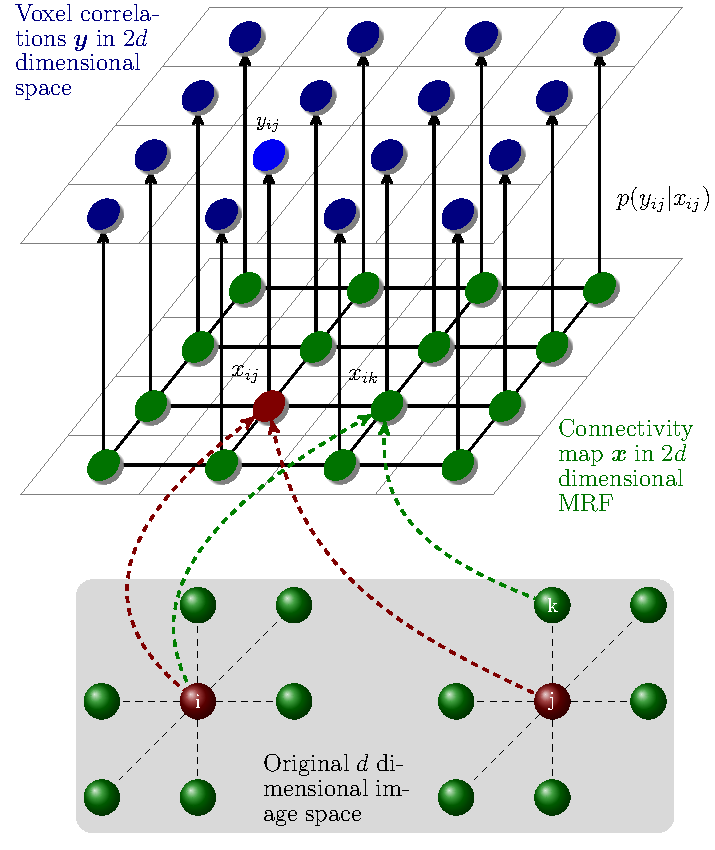
\includegraphics[width=0.4\textwidth]{figures/6dmrf}
  \caption{A MRF defined on high dimensional graph that model the pairwise
  connections of gray matter voxels. A node in the high dimension graph is
  defined as a pair of voxels in original image. an edge are added when any
  voxels in the two pair of voxels are spatially neighbors. This MRF is embedded
  into a generative model as a prior distribution, i.e. we suppose , a sample
  correlation is \emph{generated} from the given random variable of connectivity
  or no connectivity. For inference of the connectivity given the observed
  sample correlation data, \emph{Maximum a Posteriori} is used, together with
  the Gibbs Sampling and mean field theory approximation. }
  \label{fig:6dmrf}
\end{SCfigure}


Independent Component analysis (ICA) methods look for statistically independent
components without the need of selecting ROI~\cite{calhoun2001spatial}. But
users need to manually select meaningful component by visual
inspection. Clustering-based methods partition the brain voxels into distinct
regions (clusters), and voxels in same regions belong to same functional
networks. If the goal is to discriminate the patients and healthy control
groups, pattern classification method can also be used.

There are also graph theory based methods that treats each ROI (or voxel) as a
node on the graph, and the connectivity between them as edges, and a rich set of
graph algorithms can be used to learn the graph structure (small-worldness,
modularity, etc). 


\section{Methodology and Preliminary work} 
The main technical tool used in our series of work is the generative
probabilistic model and Markov random field (MRF). To be specific, define a graph
$\mathcal{G} = (\mathcal{V}, \mathcal{E})$, where $\mathcal{V}$ is the set of
nodes, with each node representing a single voxel in the image.  An edge
$e=(s,r)$ is added to $\mathcal{E}$ if the node $s$ and $r$ are spatial
neighbors. The label of functional network that a voxel belongs to is defined by
the random variable $x_s \in \mathcal{L} = \{1,\dots, L\}$ that attached to each
vertex $s\in \mathcal{V}$.

Two labels are correlated if they are spatially neighbor. The network label map
$x = (x_1, \dots, x_N)$ is a MRF because given the spatial neighbors of a voxel,
its network label does not depend on the remaining voxels statistically. This
local neighboring structure can be represented globally by a multivariate
distribution

\begin{equation*}
  Prob(x) = \frac{1}{Z}\exp\left\{-\beta \sum_{(s, r)\in\mathcal{E}} \delta(x_s, x_r)\right\}.
\end{equation*}
The function $\delta(x_s,x_r)$ takes 1 when $x_s = x_r$, and takes 0
otherwise. By this definition, a label map with large regions of constant labels
has higher probability. This will be used as a regularization prior in our
Bayesian model. The applications of MRF in my work depends on the specific
questions to answer. In \cite{liu2010spatialCopy}, it is used as a prior
distribution of a high dimensional MRF. In \cite{liu2011monteCopy}, it is used in a
generative model for clustering. And in \cite{Liu2012aCopy}, the MRF is
generalized to include both group labels and subject labels for solving a joint
estimation problem.

\subsection{Full Pairwise Connectivity With Spatial Coherence}\label{sec:highmrf}
Our first attempt~\cite{liu2010spatialCopy} on detecting functional network aims to
explicitly model the spatial smoothness of the network. In both task-based and
resting-state fMRI the impact of imaging noise can be reduced by taking
advantage of the spatial correlations between neighboring voxels in the image. A
common approach used for instance in statistical parametric mapping
(SPM)\cite{worsley_analysis_1995} is to apply a spatial Gaussian filter to
smooth the signal prior to statistical analysis. However, this can lead to
overly blurred results, where effects with small spatial extent can be lost and
detected regions may extend beyond their actual boundaries. An alternative
approach to spatial regularization that has been proposed for task activation
paradigms is to use a Markov Random Field (MRF)
prior~\cite{ou_spatial_2005,descombes_spatio-temporal_1998,descombes_fmri_1998,woolrich_fully_2004,cosman_exact_2004},
which models the conditional dependence of the signals in neighboring voxels.

We propose~\cite{liu2010spatialCopy} to use MRF models in rs-fMRI to leverage spatial
correlations in functional connectivity maps. Unlike previous MRF-based
approaches, which use the neighborhood structure defined by the original image
voxel grid, the neighborhoods in functional connectivity must take into account
the possible relationships between spatially distant voxels. Therefore, we
define the neighborhood graph on the set of all voxel pairs. This results in a
Markov structure on a grid with twice the dimensions of the original image data,
i.e., the pairwise connectivities for three-dimensional images results in a
six-dimensional MRF. The neighborhood structure is defined so that two voxels
are more likely to be connected if they are connected to each other's spatial
neighbors. See figure \ref{fig:6dmrf} for a illustrative view.


We combine the Markov prior on functional connectivity maps with a likelihood
model of the time series correlations in a posterior estimation problem.
Furthermore, we model solve for the unknown parameters of the MRF and likelihood
using an Expectation Maximization (EM) algorithm. In the estimation step the
posterior random field is sampled using Gibbs Sampling and estimated using Mean
Field theory.

Fig.~\ref{fig:mrfvssmoothing} compares the real data results using no spatial
regularization, Gaussian smoothing, and the proposed MRF model. Though the
posterior connectivity of the MRF is computed between every pair of voxels
within a slice, for visualization purposes, only the posterior of the
connectivity between one voxel and the slice is shown. We chose to visualize the
connectivity to a voxel in the posterior cingulate cortex (PCC) because this is
known to be involved in the Default Mode Network~\cite{raichle2001}, with
connections to the medial prefrontal cortex (MPFC). The results show that
Gaussian smoothing is able to remove noise, but is unable to find a clear
connection between the PCC and the MPFC. Our proposed MRF model (rightmost plot)
is able to remove spurious connections, and also clearly shows a connection to
the MPFC.

It is noted that this approach does not need \emph{a priori} knowledge of the
ROI. Once the algorithm finishes, it outputs all the pairwise connectivity for
all gray matter voxels. Putting this large connectivity matrix into a
visualization tool, users can explore the functional networks with various seed
regions and see the real-time results.

\begin{figure}[thb]
  \centering
  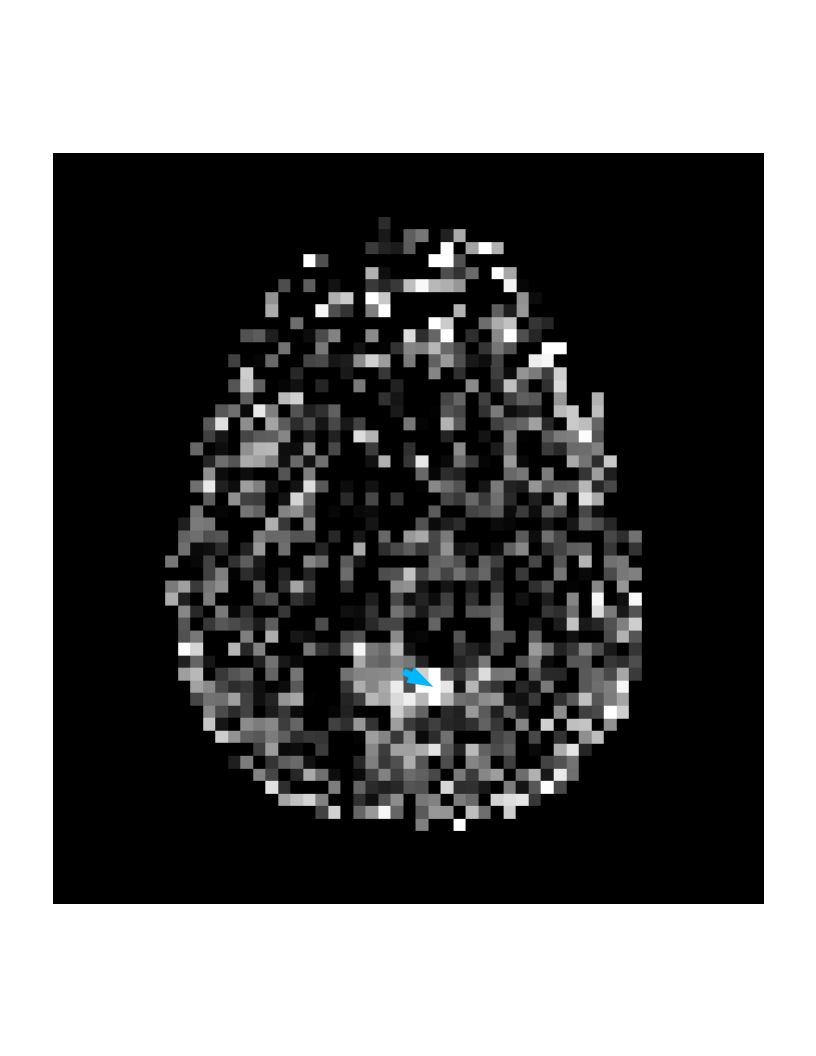
\includegraphics[width = 0.2\textwidth]{figures/no_overlay/R1_corr_nosmooth}
  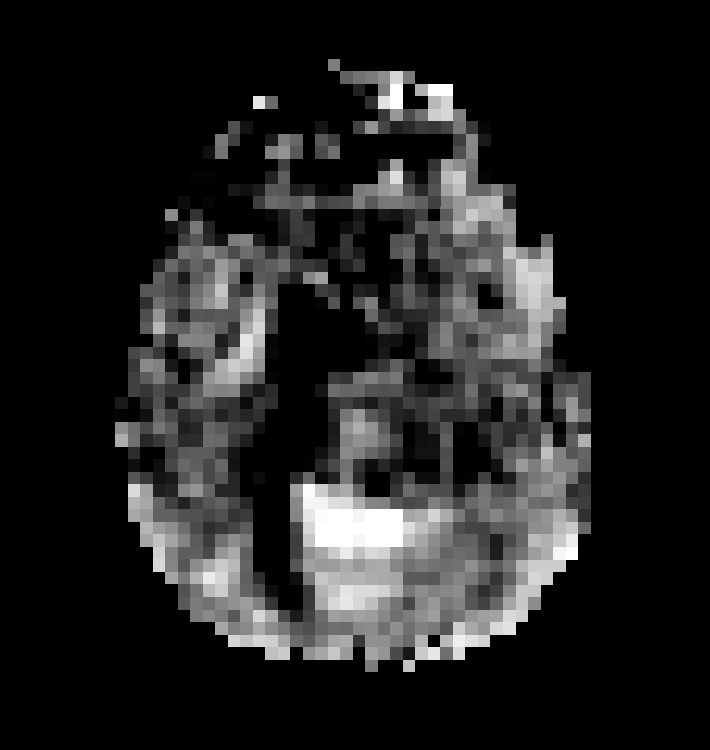
\includegraphics[width = 0.2\textwidth]{figures/no_overlay/R1_corr_smooth}
  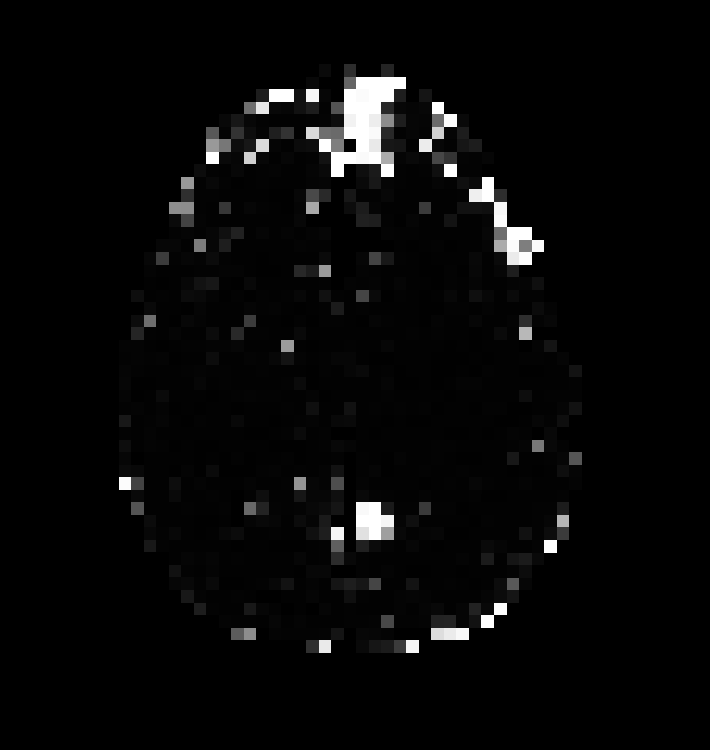
\includegraphics[width = 0.2\textwidth]{figures/no_overlay/R1_mrf}
  \caption{Correlation map and Posterior Connectivity map between seed voxel
    and slice containing the seed. From left to right: the correlation
    map computed from data without spatial smoothing;  correlation map of
    data after smoothing; Posterior probability computed from MRF.}
  \label{fig:mrfvssmoothing}
\end{figure}

\subsection{Identify Consistent, Spatially Coherent Multiple Functional Networks}

The above method in section \ref{sec:highmrf} is able to detect functional
networks such as default mode network, there are two issues that have to be
addressed. 1) With one seed region at a time, only one functional system can be
shown. The functional architecture would be better understood if multiple
systems are shown together in the same image. 2) The computation cost is huge,
mostly due to the high dimensional graph and the optimization problem.  This is
partly mitigated by a GPU implementation in current single subject analysis, but
would be difficult for generalizing to group study.

One possible solution is to employ clustering techniques to automatically
partition the brain into functional networks. In such methods, a similarity
metric is defined first, e.g., correlation \cite{5074650} or frequency coherence
\cite{thirion2006detection}, and then a clustering method such as $k$-means or
spectral clustering is used to group voxels with similar time series. A drawback
of these approaches is that they disregard the spatial position of voxels, and
thus ignore the fact that functional networks are organized into sets of
spatially coherent regions.

We introduce a new data-driven method~\cite{liu2011monteCopy} to partition the brain
into spatial coherent, non-overlapping networks of functionally-related regions
from rs-fMRI. The proposed algorithm does not require specification of a seed,
and there is no ad hoc thresholding or parameter selection. We make a natural
assumption that functionally homogeneous regions should be spatially
coherent. Our method incorporates spatial information through a Markov random
field (MRF) prior on voxel labels, which models the tendency of spatially-nearby
voxels to be within the same functional network.

We notice the mean intensity and the variance (both over all the time points) of
the time course at each voxel is not a indicator whether they belong to same
functional network, so each time series is first normalized to zero mean and unit
norm, which results in data lying on a high-dimensional unit sphere. We then
model the normalized time-series data as a mixture of von Mises-Fisher (vMF)
distributions \cite{banerjee2006clustering}. Each component of the mixture model
corresponds to the distribution of time series from one functional network.

Solving for the parameters in this combinatorial model is intractable, and we
therefore use a stochastic method called Monte Carlo Expectation Maximization
(MCEM), which approximates the expectation step using Monte Carlo
integration. The stochastic property of MCEM makes it possible to explore a
large solution space, and it performs better than a standard mode approximation
method using iterated conditional modes (ICM).

The proposed method is related to previous approaches using MRFs to model
spatial relationships in fMRI data. Descombes et
al.~\cite{descombes_spatio-temporal_1998} use a spatio-temporal MRF to analyze
task-activation fMRI data. Our previous methods~\cite{liu2010spatialCopy} use an MRF
model of rs-fMRI to estimate pairwise voxel connections. However, neither of
these approaches tackle the problem of clustering resting-state fMRI into
functional networks.

The linear correlation between two time series in original image space is
equivalent to the inner product of two points on the sphere.  MRF is again used
as a spatial smoothness prior on the hidden network labels. We estimate the
network labels by maximizing its posterior probability in a EM framework, such
that voxels with same estimated labels have larger inner product, which amounts
to have larger correlation in original space and belong to same functional
network. The introduction of MRF again poses the difficulty of computing the
expectation directly, We use Monte-Carlo Sampling to approximate the expectation
value in EM. By this method~\cite{liu2011monteCopy} we are able to detect most
significant brain networks like motor, visual, motion, salience and executive
control, and default mode network with precision and consistency competitive to
standard ICA method, as can be found in figure \ref{fig:wholebrain}.

\begin{figure}[htb]
 \begin{center}
 \begin{tabular}{cccccc}
      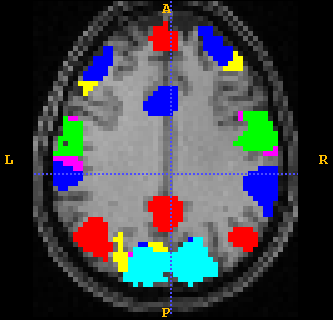
\includegraphics[width=0.1\textwidth]{figures/wholebrain/sub1/axial0028} &
      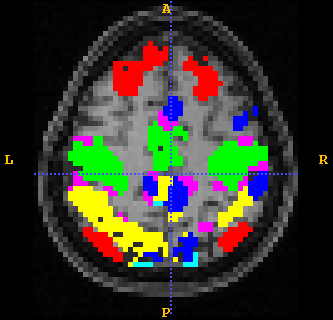
\includegraphics[width=0.1\textwidth]{figures/wholebrain/sub1/axial0034} &
      %% \vspace{0.5pt}
      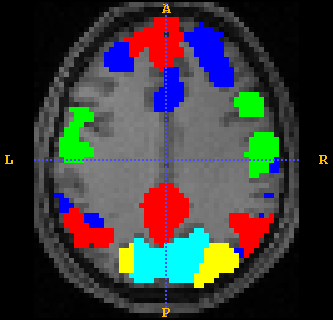
\includegraphics[width=0.1\textwidth]{figures/wholebrain/sub2/axial0028} &
      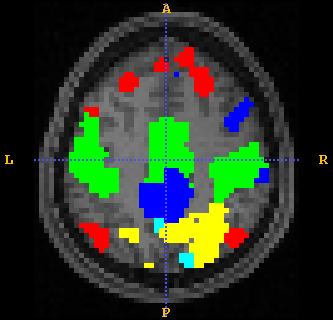
\includegraphics[width=0.1\textwidth]{figures/wholebrain/sub2/axial0034} &
      %% \vspace{0.5pt}
      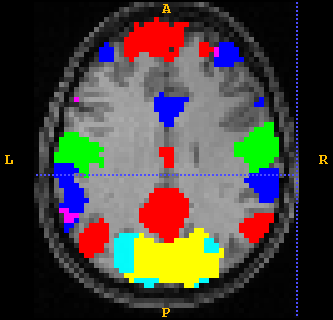
\includegraphics[width=0.1\textwidth]{figures/wholebrain/sub5/axial0028} &
      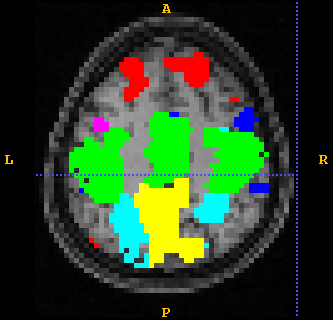
\includegraphics[width=0.1\textwidth]{figures/wholebrain/sub5/axial0034} \\

      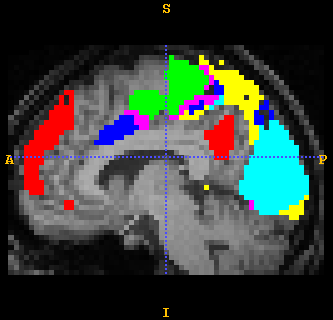
\includegraphics[width=0.1\textwidth]{figures/wholebrain/sub1/saggital0029} &
      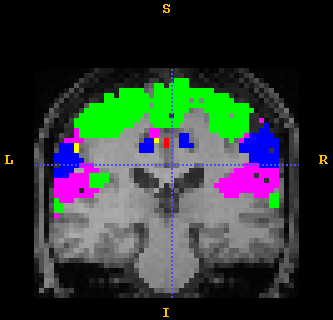
\includegraphics[width=0.1\textwidth]{figures/wholebrain/sub1/coronal0029} &
      %% \vspace{0.5pt}

      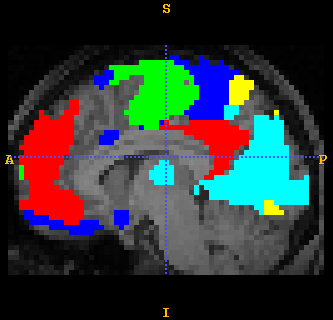
\includegraphics[width=0.1\textwidth]{figures/wholebrain/sub2/saggital0029} &
      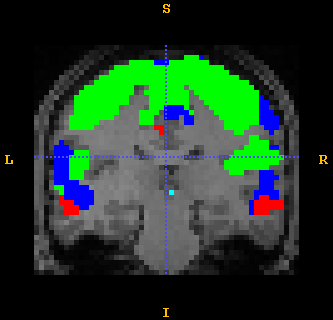
\includegraphics[width=0.1\textwidth]{figures/wholebrain/sub2/coronal0029} &
      %% \vspace{0.5pt}
      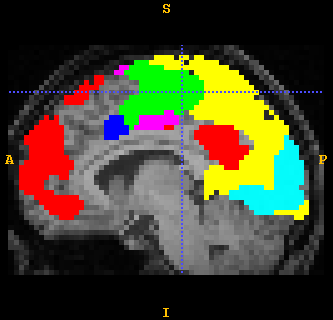
\includegraphics[width=0.1\textwidth]{figures/wholebrain/sub5/saggital0029} &
      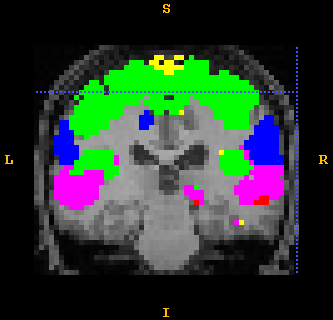
\includegraphics[width=0.1\textwidth]{figures/wholebrain/sub5/coronal0029}\\

      \multicolumn{2}{c}{\small Subject 1} &
      \multicolumn{2}{c}{\small Subject 2} &
      \multicolumn{2}{c}{\small Subject 3}
    \end{tabular}
  \end{center}
  \caption {Functional networks detected by the proposed method for 3 subjects
    overlaid on their T1 images.  The clusters are the visual (cyan), motor
    (green), executive control (blue), salience (magenta), dorsal attention
    (yellow), and default mode (red) networks.}
  \label{fig:wholebrain}
\end{figure}

\subsection{Current Work: Hierarchical Model For Group Study} \label{sec:hier}

The availability of large rs-fMRI databases opens the door for systematic group
studies of functional connectivity. It is a natural assumption that a group of
subjects must share similar patterns of functional connectivity, while keeping
individual subject's variability. Such variability may come from subject random
thoughts, despite that they are instructed not to think anything
specifically. While the inherently high level of noise in fMRI makes functional
network estimation difficult at the individual level, combining many subjects'
data together and jointly estimating the common functional networks is more
robust. However, this approach does not produce estimates of individual
functional connectivity. Such individual estimates are an important step in
understanding functional networks not just on average, but also how these
networks vary across individuals.

The method we propose in above section \cite{liu2011monteCopy} works specifically on
single subject analysis, and my next aim is to build a model that estimate
functional networks among a group of subjects.  Most current studies estimate
the networks in a sequential approach, i.e., they identify each individual
subject's network independently to other subjects, and then estimate the group
network from the subjects networks. This one-way flow of information prevents
one subject's network estimation benefiting from other subjects.

Group ICA \cite{calhoun2001spatial} is a generalization of ICA to multiple
subjects, in which all subjects are assumed to share a common spatial component
map but have distinct time courses. The time courses from all subjects are
concatenated temporally, followed by a single ICA. Although the subject
component maps are obtained by a back-reconstruction procedure, there is no
explicit statistical modeling of the variability between the group and subject
component maps.  Ng et. al \cite{nggroup2012} use group replicator dynamics (RD)
to detect subject's sparse component maps, with group information integrated
into each subject's RD process. In clustering-based methods, the subjects
clusterings are usually averaged to obtain a group affinity matrix and are
followed by a second level clustering on the group similarity matrix
\cite{bellec2010multi,van2008normalized}. Because the group level clustering is
conducted after subject level clustering, the clustering of one subject is
unaware of the information from other subjects, as well as the group clustering.


%% \begin{figure}[htb]
%%   \centering
%%   \begin{tabular}[b]{c}
%%     \includegraphics[width=0.25\textwidth]{figure1/grp2}
%%   \end{tabular}
%%   \hspace{5pt}
%%   \begin{tabular}[b]{c}
%%     \begin{tabular}[b]{lccccc}
%%       & \footnotesize Truth & \footnotesize \textsf{K-Means} & \footnotesize \textsf{N-Cuts} & \footnotesize \textsf{groupmrf}\\
%%       \begin{sideways} \footnotesize group \end{sideways} &
%%       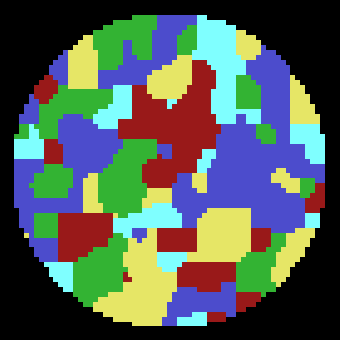
\includegraphics[width=0.1\textwidth]{figure1/truegrp} &
%%       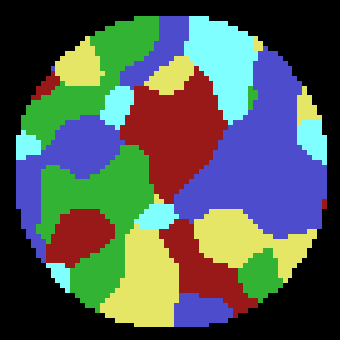
\includegraphics[width=0.1\textwidth]{figure1/kmeans_grp} &
%%       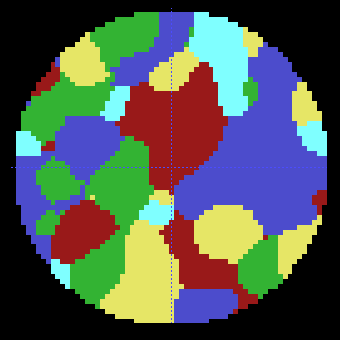
\includegraphics[width=0.1\textwidth]{figure1/ncuts_grp} &
%%       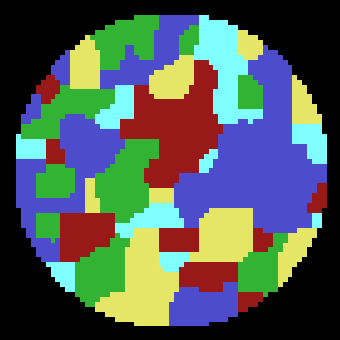
\includegraphics[width=0.1\textwidth]{figure1/mrf_grp} \\
%%       \begin{sideways} \footnotesize sub 1 \end{sideways} &
%%       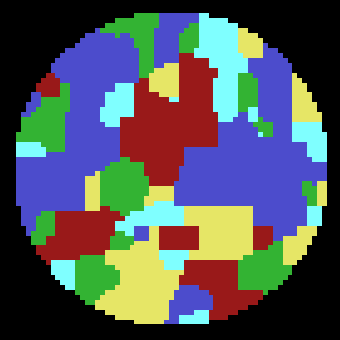
\includegraphics[width=0.1\textwidth]{figure1/true_sub1} &
%%       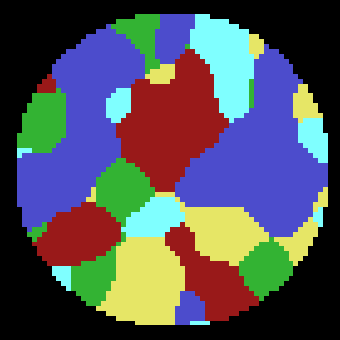
\includegraphics[width=0.1\textwidth]{figure1/kmeans_sub1} &
%%       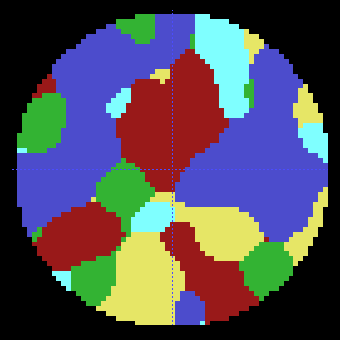
\includegraphics[width=0.1\textwidth]{figure1/ncuts_sub1} &
%%       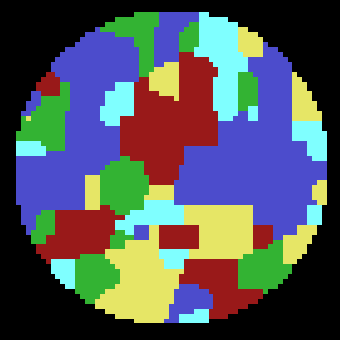
\includegraphics[width=0.1\textwidth]{figure1/mrf_sub1} \\
%%     \end{tabular} \\
%%     \hspace{15pt}
%%     \footnotesize
%%     \begin{tabular}[b]{l|ccc}
%%       & group & mean(sub) & var(sub) \\
%%       \textsf{K-means} & 92.9 & 87.0 & 0.67\\
%%       \textsf{N-Cuts} & 85.4 & 87.1 & 0.58 \\
%%       \textsf{groupmrf} & 95.7 & 97.5 & 0.59
%%     \end{tabular}
%%   \end{tabular}
%%   \caption{Left: Hierarchical MRF depicted by undirected graph. The $J$ subjects
%%     are compactly represented by a box with label $J$. Right: clustering of
%%     \textsf{K-means} and \textsf{N-Cuts} on synthetic time series with spatial
%%     smoothing, and \textsf{groupmrf} without smoothing. Top is group label map
%%     and bottom is one of subjects label map. The table gives the rand index accuracy
%%     between estimated label map and ground truth image. The rand index of all
%%     subjects are summarized by a mean and variance value.}
%%   \label{fig:fig1}
%% \vspace*{-8pt}
%% \end{figure}


\begin{figure}[htb]
  \centering
  \begin{tabular}[b]{c}
    \includegraphics[width=0.25\textwidth]{figure1/grp2}
  \end{tabular}
  \caption{Left: Hierarchical MRF depicted by undirected graph. The $J$ subjects
    are compactly represented by a box with label $J$. $\alpha$ and $\beta$ are
    parameters that represent the strength of the statistical dependencies
    between the nodes.}
  \label{fig:fig1}
\vspace*{-8pt}
\end{figure}

We propose a Bayesian hierarchical model~\cite{Liu2012aCopy} to identify the
functional networks from rs-fMRI that includes both subject and population
levels. We assume a group network label map that acts as a prior to the label
maps for all subjects in the population. This Bayesian perspective provides a
natural regularization of the estimation problem of a single subject using
information from the entire population. The variability between the subjects and
group are taken into account through the conditional distributions between group
and subjects. The within-subject spatial coherence is again modeled by a
MRF. The group and all subjects network map are connected into a larger graph,
with edges between corresponding voxels between group and subjects, and between
adjacent voxels within single subjects. See figure \ref{fig:fig1} for the model
illustration.

The concept of this hierarchical model is similar to the multi-level modeling of
linear regression. Estimation of the functional network on single
subject corresponds to no pooling since it fits a model for each subject
separately. A sequential approach of estimating group network after subjects
networks is like complete pooling, since it ignores the group information when
estimating subjects network. And our hierarchical MRF model corresponds to the
partial pooling, i.e., the multi-level model where a tradeoff defined by a
pooling factor, or a shrinkage factor. Compared to the \emph{pooled} averaging
method, our hierarchical model respects the individual variablity, hence also
better estimates the group's functional network.

Both the group clustering and subject clusterings are estimated simultaneously
with a Monte Carlo Expectation Maximization (MCEM) algorithm.  The model is
data-driven in that all parameters, regularized by two given hyper-parameters,
are estimated from the data, and the only parameter that must be specified is
the number of networks.

Ours is the first hierarchical MRF applied to fMRI for modeling both
group and individual networks. The model of Ng et al. \cite{ng2010group}
combines all subjects into a single MRF and bypasses the need for one-to-one
voxel correspondence across subjects, but the edges are added directly between
subjects without a group layer. In our model, a group layer network map is
explicitly defined, and the consistency between subjects is encoded through
adding edges between group and subjects labels. Our method differs from other
clustering methods \cite{bellec2010multi,van2008normalized} in that their
methods identify the subject's functional network patterns independently,
without any knowledge of other subjects or group population. Instead, our method
estimates both levels of network patterns simultaneously.  The proposed approach
can be seen as a counterpart on the clustering branch of the multi-subject
dictionary learning algorithm \cite{varoquaux2011multi}, which also has a
hierarchical model and a spatially smoothed sparsity prior on the group
component map.

\subsection{Variability of Resting-State Functional Network}
The hierarchical MRF model decreases the scanner noise, physiological noise and
other artifacts, but does not spoil the true signal. The variability of the
functional connectivity due to individual subject's spontaneous thoughts is
believed to be part of the true signal that we want to keep and explore. Given
the Bayesian model we proposed in section \ref{sec:hier}, a multivariate
posterior distribution of the connectivity variables is available as a summary
of our current state of knowledge (arising from both the observed data and the
MRF prior opinions). A standard point estimate would just report a single value
(mean, mode or median) for each variable. However, when the sample size is
small, and number of variables is large (which is the case in fMRI study), it is
inappropriate to summarize inference by one value, especially when the summary
is used for clinical decision. We need to measure the uncertainty and
variability of the estimates. Uncertainty means the variance of the connectivity
variables inferred from the posterior density. Variability means the change of
the spatial patterns because of single variable's uncertainty and the difference
across subjects.

Because the lack of analytic solution of posterior distribution, obtaining the
uncertainty of single variable is not straightforward. However, by using the
Markov Chain Monte-Carlo tool we developed in previous work, we are able to
draw samples of the connectivity variables from the posterior, and estimate the
variance from the samples. 

Given the uncertainty on the voxel level, the more interesting question is the
variability on the network level. Here I want to find the most dominant pattern
of  change of a functional network over subjects, as well as over the
uncertainty of single voxels. For example, does the PCC's size and shape change
over all subjects mainly happen along the dorsal-ventral direction, or the
anterior-posterior direction? We can see the functional network patterns as
objects with certain shape and size. The change of the shape or size can be
represented by the multivariate analysis method such as principal component
analysis.


%%  especially the multivariate
%% posterior distribution is multi-mode. 

%% Currently our model has a parameter that controls how much the subject function
%% network maps should \emph{shrink} towards the group network map. I aim to find
%% some guidance of how to set the parameter value based on either the data itself
%% or some physiology knowledge.

%% Another interesting question I want to explore is the convergence of the Markov
%% chain. The inference of posterior from the hierarchical model that we proposed
%% in \cite{Liu2012aCopy} poses a difficult optimization problem, and a Markov
%% Chian Monte Carlo (MCMC) method is used to obtain approximate solution. In
%% general Markov Chain sampling, some convergence tests are available
%% \cite{cowles1996markov} as guidance of when to stop the chain. However, since
%% MCMC on MRF is a multivariate problem, it is difficult to have a stopping rule
%% to guarantee that the number of iterations is sufficient. My aim is to find a
%% method that can give a bound of the required iterations before the samples are
%% from the stationary distribution. One method is the coupling technique
%% \cite{haggstrom1999exact,propp1996exact}, where two or more parallel chains are
%% sampled based on same sequence of random number. The sampling procedure
%% converges when all the parallel chains coupled, i.e. reach to same state.

\section{Timeline} 
Based on the my current work and the contributions that I will work on, I give
the schedule for the remaining time of the thesis work:
\begin{itemize}
  \item \textbf{Fall 2012:} Network variability analysis.
  \item \textbf{Spring 2013}: Submit a journal paper on the hierarchical model
    in section \ref{sec:hier}. Continue on variability analysis.
  \item \textbf{Summer 2013}: Dissertation writing and Ph.D thesis defense.
\end{itemize}


\bibliographystyle{unsrtnat}
\bibliography{/home/sci/weiliu/projects/centralref}

\appendix
\renewcommand{\refname}{List of Publications}
\begin{thebibliography}{1}

\bibitem[Liu10a]{liu2010spatialCopy}
W.~Liu, P.~Zhu, J.~Anderson, D.~Yurgelun-Todd, and P.T. Fletcher.
\newblock Spatial {R}egularization of {F}unctional {C}onnectivity {U}sing
  {H}igh-{D}imensional {M}arkov {R}andom {F}ields.
\newblock \emph{Medical Image Computing and Computer-Assisted
  Intervention--MICCAI 2010}, pages 363--370, 2010.
\newblock URL
  \url{http://www.sci.utah.edu/publications/liu10/MRF_connectivity_miccai2010.pdf}.

\bibitem[Liu11a]{liu2011monteCopy}
W.~Liu, S.~Awate, J.~Anderson, D.~Yurgelun-Todd, and P.T. Fletcher.
\newblock Monte {C}arlo {E}xpectation {M}aximization with {H}idden {M}arkov
  {M}odels to {D}etect {F}unctional {N}etworks in {R}esting-{S}tate {fMRI}.
\newblock \emph{Machine Learning in Medical Imaging}, pages 59--66, 2011.
\newblock URL
  \url{http://www.sci.utah.edu/~weiliu/publications/mcem_weiliu_miccai2011.pdf}.

\bibitem[Liu12a]{Liu2012aCopy}
W.~Liu, S.~Awate, and P.T. Fletcher.
\newblock Group analysis of resting-state {fMRI} by hierarchical {M}arkov
  {R}andom {F}ields.
\newblock \emph{MICCAI 2012}, In Press.
\newblock URL
  \url{http://www.sci.utah.edu/~weiliu/publications/hiermrf_miccai12.pdf}.

\end{thebibliography}


\end{document}
